% !TeX spellcheck = en_US
% !TeX encoding = UTF-8

% COMPILE WITH:
% `latexmk`
% You need lualatex and biber (in all TeXLive distributions)

\documentclass[
    numbers=noenddot,
    %listof=totoc,
    parskip=half-,
    fontsize=12pt,
    paper=a4,
    oneside,
    titlepage,
    bibliography=totoc,
    chapterprefix=false,
%    draft
]{scrbook}

% use lualatex or xelatex
%\usepackage{fontspec}
\usepackage{graphicx}
\usepackage[onehalfspacing]{setspace}

% better language support
%\usepackage{polyglossia}
%\setdefaultlanguage{english}
%\setotherlanguage{german}

\usepackage{tocbasic}
\usepackage{booktabs}
\usepackage{multicol}
\usepackage{multirow}
\usepackage{amsmath}

\usepackage[]{scrlayer-scrpage}

% better bibliography (biblatex style)
% use biber to compile
\usepackage[citestyle=alphabetic, bibstyle=alphabetic, sorting=nyt, backend=biber, language=english, backref=true, maxcitenames=2]{biblatex}

% better quotes
% use \enquote{text}
\usepackage[autostyle,english=american,german=quotes]{csquotes}
\addbibresource{bibliography.bib}

% appendix
\usepackage[titletoc]{appendix}

% where to put all images and figures
\graphicspath{{images/}}

% YOUR PACKAGES


% Title
\title{Analysing and Mining geo-locational data from tweets for understanding people opinion on migration}

% Author
\author{Pooran Chandrashekaraiah}

% Date
\date{\today}

% CHOOSE ACCORDINGLY
%\newcommand{\thesisType}{Bachelorarbeit}
\newcommand{\thesisType}{Masterarbeit}

\makeatletter
\let\thetitle\@title
\let\theauthor\@author
\let\thedate\@date
\makeatother

\pagestyle{scrheadings}

\begin{document}

%%%%%%%%%%%%%%%%%%%%%%%%%%%%%%%%%%%%%%%%%%%%%%%%%%%%%%%%%%%%%%%%%%%%%%%%%%%%%%%%%%%%%%%%%
\frontmatter
% CHOOSE ACCORDINGLY
%% !TeX spellcheck = en_US
% !TeX encoding = UTF-8
\begin{titlepage}
    \centering
    \begin{onehalfspace}
    
        	
\includegraphics[width=7cm]{uni-logo.png}\\
        	\vspace{1.0cm}
        	\large {\bfseries Lehrstuhl für Data Science \\

        	\vspace{2.5cm}

            \begin{doublespace}
            	{\textsf{\Huge{\thetitle}}}
            \end{doublespace}

        	\vspace{2cm}

            \Large{Bachelorarbeit von}\\

        	\vspace{1cm}

        	{\bfseries \large{\theauthor}}

        	\vfill

        	{\large
        		\begin{tabular}[l]{cc}
        			\textsc{Prüfer}\\
        			Prof.~Dr.~Michael Granitzer
        		\end{tabular}
        	}

        	\vspace{1.5cm}

        	\parbox{\linewidth}{\hrule\strut}

            \vfill

	    {\thedate}
    	
    \end{onehalfspace}
\end{titlepage}

% !TeX spellcheck = en_US
% !TeX encoding = UTF-8
\begin{titlepage}
    \centering
    \begin{onehalfspace}
    	
        	
\includegraphics[width=7cm]{uni-logo.png}\\
        	\vspace{1.0cm}
        	\large {\bfseries Lehrstuhl f\"ur Data Science }\\

        	\vspace{2.5cm}

            \begin{doublespace}
            	{\textsf{\Huge{\thetitle}}}
            \end{doublespace}

        	\vspace{2cm}

            \Large{Masterarbeit von}\\

        	\vspace{1cm}

        	{\bfseries \large{\theauthor}}

        	\vfill

        	{\large
        		\begin{tabular}[l]{cc}
        			\textsc{1.~Pr\"ufer} & \textsc{2.~Pr\"ufer} \\
        			Prof.~Dr.~Michael Granitzer& Prof.~Dr.~Harald Kosch
        		\end{tabular}
        	}

        	\vspace{1.5cm}

        	\parbox{\linewidth}{\hrule\strut}

            \vfill

	    \thedate
    \end{onehalfspace}
\end{titlepage}


\tableofcontents
\newpage

% -- ABSTRACT
% !TeX spellcheck = en_US
% !TeX encoding = UTF-8
\chapter*{Abstract}
The objective of this thesis is to initially classify the tweets as human migration tweet or not. And then detect the sentiment of the classified migration tweet.  People use the tweets, which are a short message to express their opinion on the topic they are interested in. Which makes, interesting and challenging to classify these tweets to specific classes. Migration classifier classifies tweets into "migrations" or "not migrations" classes and sentiment classifier classifies the sentiment of the tweet into "positive" or "negative" classes. The binary classifier is built using a supervised machine learning algorithm.

Set of supervised classifier algorithm consisting of logistic regression, naive Bayes, decision trees are used to create the classification model.  However, the data required to create these classifiers should be preprocessed and features extracted. The count vector and the presence of migration terms are used as the feature vector for the migration detection model, while only the count vector is used as the feature vector for the sentiment detection model. The performance of the learned classifier model is then calculated using the test data.

The dataset for the migration detection model is self-built by searching the data archive using hashtags and manually annotating the labels.  An annotated dataset with the positive and negative labels is used for sentiment analysis. Accuracy and the F1-score of both the models were pretty good, however, when the migration tweets from the migration detection model are sent to sentiment detection model, the prediction was approximately 55\% accurate.

\textit{Keywords: Data analysis, text mining, classification, sentiment analysis, twitter}
\newpage

% -- Acknowledgements (optional)
% !TeX spellcheck = en_US
% !TeX encoding = UTF-8
\chapter*{Acknowledgments}

% I would first like to thank my thesis advisor ...
\newpage

% -- List of figures
\thispagestyle{empty}
\cleardoublepage
\listoffigures
\newpage

% -- List of tables
\thispagestyle{empty}
\cleardoublepage
\listoftables
\newpage

%%%%%%%%%%%%%%%%%%%%%%%%%%%%%%%%%%%%%%%%%%%%%%%%%%%%%%%%%%%%%%%%%%%%%%%%%%%%%%%%%%%%%%%%%
\mainmatter

% -- Chapters
% following IMRaD structure
% adjust for your liking
\chapter{Introduction}\label{chap:introduction}
Migration is one of the social phenomena in human beings life. It is the physical movement of human beings from one place to another for short or long term within or state borders. The sociologist has come up with the push-pull model after lots of research. This model tells or compares the push factors, that usually happens when sending country forces people to leave their homes, to pull factors, which attracts the people onto receiving country. In recent history, the reasons for migration has changed and its changing. Today people migrate as an asylum seeker or as a trafficked person or refugee or as an international student.

Data Regarding migration flows are largely inconsistent across countries, typically outdated and
are often nonexistent. Research on migration policy making from International Organization for
Migration(IOM)  \cite{IOM's} quotes "Migration has become one of the most challenging issues confronting
policymakers around the world. The growing complexity of internal and cross-border human mobility
has highlighted the need for reliable and timely data to inform migration policy development
and humanitarian assistance". 

Migration data is one the important parameter for demographic changes, But the traditional methods of collecting and storing data of migration statistics are limited. The census which is the comprehensive source of information about the entire population usually takes place every 5 to 10 years, some data is lost between census cycles. Methods like census and population registers may often not be appropriate to estimate short-term migration. 

Spread of internet application, social media, and mobile phones as massively effected on how we communicate with others. \cite{Christina_Hughes_et_al.} discusses about the traditional and new approaches of gathering human migration data. This has helped many researchers to study on societies and due to the Digital revolution, these data are stored. The key features in these data are Time and Geo-location. Availability of Spatial-Temporal data from online sources has opened up new opportunities for the data scientist. These data can be accessed by anyone with relevant technical skills like Twitter data-sets, Linked-In data-sets, mobile phone data or can be bought from companies like Google and Facebook (they don't sell the user data). Mainly, the data collected is based on the data desired. "Time" would be one of the important parameters to estimate the migration trends. Along with that, a specific group of population data (example: "Refugee") could be used to analyze trends. Human migration flow based on political reason, short-term migration for Education, employment and gender can be used to collect data. Twitter is widely accepted all over the world and people use this forum to communicate all types of views and opinion, in this research, the extraction of the topic specifically to human migration from a tweet is studied. 


\cite{Cortis} has proposed a successful approach for identifying tweets associated with the subject "cyberbullying". Our approach differs from the approach mentioned, as the subject of the tweet is human migration. Since Twitter is widely used in all strata, it can be regarded as a good picture of what is happening worldwide.  Our assessment shows that people express their opinions on all trending topics. Of all topics, politics, war and human migration are the focus of this research. These data can be analyzed to understand the opinion of the people who tweet about human migration.  With the focus on mining Twitter data and gathering information on a specific topic which is Human migration in my research. I need to understand why people migrate and implement a strategy to mine migration tweets. Once the Tweets are classified as migration tweets, these tweets are used to understand the sentiment of the people who are tweeting this. So the work in my thesis concentrates on following questions.


  

\begin{itemize}
  \item A framework to classify Tweets which are related to human migration.
  \item Detect the sentiment of the migration classified tweets. 
\end{itemize}

This paper is organized as follows: chapter \ref{chap:background}  provides the background of the different related fields.
The main topics that are discussed are: Twitter data analysis, Text mining and classification algorithms and related work and in chapter \ref{chap:approach} we describe problem formulation and methods used in this research.
approach and its concrete implementation. The results are
presented in Section 4, accompanied by an empirical analysis of computer scientists on Twitter in Section 5. We draw
conclusions about our approach in Section 6.


In this 


\underline{brief agi bari about the approach}


\chapter{Background}\label{chap:background}
This chapter displays the background of the investigation, to enable a better comprehension of the framework executed. It starts with an introduction to the Twitter API's, and data structure used by Twitter, followed by Text mining, classification algorithms, metrics to measure classification algorithms. The accompanying segment focuses on the past work that has been done in the field of mining Twitter's information and its analysis.

machine learning pipeline, data crawling, and stuff
    
\section{Technical Background}

The core task of detecting the Sentiment of the Tweets which are related to ``Human Migration" requires techniques related to Data mining, Text mining and Machine Learning. For instance, typical Data analysis systems first extract Data regarding the ``Human migration" from the tweets, and supervised classifier such as logistic regression or Naive Bayes or decision trees  are used for classification and detection. Thus, Data mining and classifier algorithms are the core tools in this computation analysis and hence are covered in this section.

\subsection{Twitter Data analysis}

Twitter is one of the well known online social networks, People use this to communicate short messages (140 character length) called tweets and express opinion on various topics that they are interested in. It is also called ``Microblogging", which is different from other social media platform like Facebook. One more thing which makes Twitter different from Facebook is, Networking is not bidirectional. Which means connections don't have to be mutual. Another  potential aspect of choosing Twitter for mining data is, It popularized the term hashtags. Which is used to group a  conversation and user can follow a particular topic.

Twitter provides a number of APIs to collect Twitter data programmatically. \cite{TwitterDevDocs} Gives a complete list of all Twitter APIs and the steps to set up the project to access Twitter data. Data from these APIs can be collected by more than one way, which can be broadly categorized as REST APIs and Streaming APIs . But, Twitter API limits access to applications. The rate limits are described in link  \footnote{https://developer.twitter.com/en/docs/basics/rate-limiting}. Usually, the REST APIs are used to search for the existing tweets or tweets which are already published. These APIs are not only rate limited also they are limited based on the time span (search tweets back to one week). Then, the streaming APIs can be used to collect tweets as per our search criteria and as they publish in current time(example: live events). These APIs are rate limited on a per-user basis. Based on the two limitations mentioned above, we choose to use the Twitter data archive \footnote{https://archive.org/details/twitterstream?and[]=year\%3A\%222016\%22}. This has given me the advantage of selecting archives based on a certain time frame.



\cite{Marco} Gives in-detail about how the data in Twitter are represented
and how the data can be extracted. Sample structure of the tweet JSON(JavaScript object notation) is shown in the figure \ref{fig:Tweet_json}. Twitter contains Hashtags, Topics and Time Series along with
Users, Followers, and Communities. And  \cite{Marco} also explains how to filter hashtags, represent the
tweets in graphs. Tweets are spatial-temporal data as these contain Geo-tag along with Created
Time metadata.

\begin{figure}
	\centering
	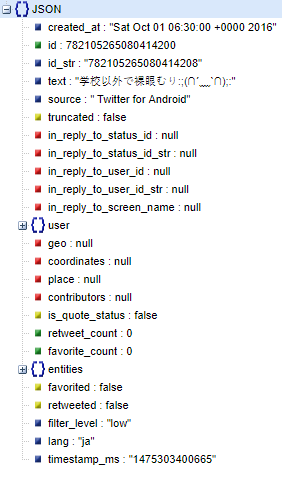
\includegraphics[width=0.5\linewidth]{thesis_template/images/tweet_json.png}
	\caption{Sample JSON of the tweet.}
	\label{fig:Tweet_json}
	
\end{figure}


 But, building a successful system to detect Human migration Tweets and predicting the opinion of these Tweets requires selecting relevant features and a suitable machine learning model. With respect to Twitter data, These are obtained as JSON format. Each object contains metadata like Hashtags, Topics, Time series, Geo-tags along with these Users, Followers, and Communities. The ``Text" metadata in the Tweet is noisy as it is only 140 characters long(recently increased to 280 characters) and people would shorten the words in an unexpected manner. Traditionally while building a machine learning model "Text" metadata has used a feature. As it has many other particular features like Mentions(@user) and Hashtags(\# topic) which provide useful information.
 
 
\subsection{Text mining}

In the Previous section, I discussed the Twitter APIs and the Twitter datasets. This subsection focuses on the techniques and processes of using the Text for classification and addition of other features along with text to improve the accuracy of the classifier algorithms.  In this chapter pre-processing of the data, the feature selection is discussed.

\subsubsection{Data Pre-processing}

Pre-processing of data is one of the main steps in any data mining experiments. This step is extensively used and studied by a lot of applications which uses unstructured, raw data. The Data that does not have a recognizable structure or less ordered is called as unstructured data.  Though we do have the data, analyzing raw format data produce misleading results if the data is not carefully screened. So, data need to be structured and formatted, which makes Data Pre-processing step important and necessary.

Usually, All the \underline{[list of the literature in the paper]} performs preprocessing on the Twitter data for their analysis. Steps,  like removing the unwanted symbols, filtering tweets, removing the stop words,  correcting errors, converting the text to lowercase are common in most of the Text preprocessing experiments.

Symbols like `@' and `\#' which are used to mention users(eg:@john) and describe the topic(eg:\#elections2018) respectively which are often present in the text of the Tweet, can be removed. Because these symbols will not give useful information while analyzing text. Just like these symbols, stop words are also removed. Stop words are the words which occur most frequently(eg: the, is, at, which, on), which are removed the from text in most of the Natural language processing projects. 

Removal of repeated data is also a significant step in text analysis. There might be a lot of repeated Tweets, Re-tweets or repeated letters in the words(example: `Greattttt', `Aweeeeesome!!!!'). A filtering technique is applied to remove or check for the similarity of tweets and avoid duplicates. In addition to this duplicate check step, one more step in every text analysis experiment is to convert the text to a lower case. The text often has a variety of capitalization reflecting the beginning of sentences, proper nouns emphasis. Which should be normalized into a single form. But care should be taken using regular expression or dictionary of words as it should not change the meaning (example: `US' to `us').

Another widely recognized method to filter strings/texts is using a regular expression \cite{Thompson}. It provides an easy way to recognize substrings, when we have the pattern to search and the text document. The regular expression search function searches the entire corpus(large and structured set of texts) and return the substring based on the pattern. A regular expression is just a special sequence of characters for identifying strings. It is now a standard feature in almost all programming language and tools which has a capacity to fit nearly all string patterns.   

Another helpful method which can be used in data pre-processing step for text is Stemming. It is a process of reducing the word to its word stem which is the original root form. An example of a stemming method is it reduces the word "cheaper" to "cheap" and "cheapest" to "cheap". This helps in reducing the number of words, in-turn aids in giving better results while analyzing the text data.

Apart from all these techniques mentioned above, Language of the text plays an important role. Different language has different grammar, set of words. As mentioned in previous methods, if the data is clean and preprocessed, accurate classifier models can be trained. If the Text from the different languages is used, a noise will be introduced later when the classifier is trained. Building a general model for all the languages will be difficult as grammar and wordset of languages differ. Model built using the English language text cannot be used on Hindi language text. Consequently, Language detection is necessary. Collecting the data of a single language can be done by two operations, either by translation or filtering. Both steps requires to process of identifying language. One simple method is to understand the distribution of the characters per language. This is one of the interesting field of research in Natural Language Processing, to identify languages. 

Once the data is collected from the same language and preprocessed, the data can be fed to feature extraction and engineering step.

\subsubsection{Feature Extraction and Engineering} \label{backgroundworkFeatureEngi}

Feature engineering is another important step in construction of an intelligent system. Although there are many new technologies, such as deep learning and meta-heuristics, that help with automated machine learning, Each problem is domain specific and better features (problem-friendly) are often the decisive factor in our system performance. This is why Data scientist spend most of the time in data preparation and feature extracting. Almost 70\% of time is spent in this step before model preparation. As famous researcher on the field of data science Andrew Ng, quotes ``Coming up with features is difficult, time-consuming, requires expert knowledge. `Applied machine learning' is basically feature engineering.". Which explains why this steps is time-consuming and difficult. This step requires both domain knowledge and mathematical computations. Another researcher Dr. Jason Brownlee, quotes ``Feature engineering is the process of transforming raw data into features that better represent the underlying problem to the predictive models, resulting in improved model accuracy on unseen data.". This explains us that perhaps feature engineering is the mechanism of converting data into features that act as variables for machine learning models to improve the overall performance of the model.

Features can be broadly categorized as Raw features and Derived features. Raw features are the one which are obtained directly from the dataset and the derived features are obtained from feature engineering. Data is available in many diverse forms like "Continuous, numeric data", "Discrete, categorical data" . Data which are stored as a scalar values, which usually represents recordings, measurements or observations are referred as Continuous, numeric data (it can also be represented as vector but each value represent a feature). Although numerical data can be effectively fed into machine learning models, we will still need to develop situation, problem and domain-relevant features before even building a model. In contrast to continuous numeric data, the categorical data attribute are represented as discrete values that belong to a certain limited set of categories or classes. which are also often referred to as classes or labels in the context of attributes or variables that a model must predict. This categorical data as two types, nominal and ordinal. In nominal attributes, There is no concept of ordering within the attribute's values(eg: zip codes, employeeIDs, eye color, gender: {male, female}). For ordinal attributes, there exist a sense or idea of order in their values(eg: hardness of minerals, grades, street numbers, quality: {good, better,
best}). Now that we have addressed the types of data representation, 
We will now understand the structure of text and text data feature engineering. As text from the tweet is used to build machine learning model. 

The importance of feature engineering is even more significant for unstructured textual data, because if we want to use text in machine learning algorithms, we need to convert it to a numerical representation. The Bag-of-word(BOW) approach is one of the methods. The bag of words is a text representation describing the occurrence of words inside a document. There are two things involved; one, a known word vocabulary and second, measure of the existence of known words. The term "Bag-of-word" is used because this model discards order of words and grammar.  Once we have a corpus( text data), This approach represents each text document as a numeric vector where each dimension is a specific corpus word and its frequency, occurrence (denoted by 1 or 0) or even weighted values. Researchers have proposed and experimented with different text features representation in the text analysis, to test which extraction methods worked well. Some features extraction methods discussed here are:  n-grams and tf-idf measure.

\paragraph{N-grams} 


A n-gram is an adjacent sequence of n words from a source of text. The n-gram method is a relatively simple algorithm. For instance, 
\begin{itemize}
  \item "Apple" - is a uni-gram(n = 1)
  \item "New York" - is a bigram(n = 2)
  \item "I love pizza" - is a trigram(n = 2)
  \item "He is walking slowly" - is a n-gram where(n = 4)
\end{itemize}
Now if we calculate the probability of a word occurring next in a sequence of words, it can be very useful. \cite{groot2012data} explains the about the n-gram and feature extraction while working on detecting the sentiment of the tweet. For unigrams where n=1, every tweet's text is split into words and each word is considered. The frequency count of all words in all documents leads to a word frequency table. High-frequency words are more likely to show up in texts, now these words better describe the dataset. Frequency can be measured among all the documents by two types such as: summed term frequency and document frequency. Summed term frequency is computed by adding all the term frequencies of the words and document frequency is number of text document the word present in. These two frequency measurements are based on term frequency and the term presence. The term frequency $tf(w,d)$ is the number of times in document $d$, a word $w$ occurs which is showed in the equation (\ref{eqn:1}). In terms frequency, we can assume the value in the [0-n] range, where n is the number of words in the document because all occurrences of a word in a document are counted for the calculation. And the term presence $tp(w,d)$ only checks whether a word $w$ is present in a document $d$, resulting in a binary value (\ref{eqn:2}).

\begin{equation}
\label{eqn:1}
tf(w,d) = |\{w \epsilon d\}|
\end{equation}
\begin{equation}
\label{eqn:2}
  tp(w,d)=\begin{cases}
    1, & \text{if $w \in d$}.\\
    0, & \text{if $w \not\in d$}.
  \end{cases}
\end{equation}
So, now the summed term frequency $stf(w,D)$ is calculated by computing the sum of all term frequencies (\ref{eqn:3}). The frequency of documents $df(w,D)$ refers to the number of documents a word occurs in (\ref{eqn:4}). The equations are referenced from \cite{groot2012data}.

\begin{equation}
\label{eqn:3}
stf(w,D) = \sum_{d \epsilon D} tf(w,d)
\end{equation}
\begin{equation}
\label{eqn:4}
df(w,D) = |\{d \epsilon D: w \epsilon d \}|
\end{equation}
Sometimes, word frequency might not give better feature sets when used in the machine learning models. In that case, higher order n-grams are used. For bigrams (where n=2), items will be two consecutive words. For trigrams (where n=3), items will be three consecutive words. But, higher the order will result in over-fitting the model. And when the document is large, the word vocabulary will be huge, so only top $k$ most valuable words will be selected.

\underline{conclude maddu, by comparing the literature survey of unigram and bigram n trigram, tell did we use ngram}

\paragraph{Count vectorizer}
Count vector is a type of word embedding based on frequency, while Word embedding format usually attempts to map a word to a vector using a dictionary. Here, the dictionary is the list of all unique words in a document. One simple way is, a vector representation of a word is a one-hot encoded vector where 1 stands for the position where the word exists and 0 everywhere else. In count vectorizer, The one-hot encoding is replaced by the frequency of words. Now, in the matrix M where rows are the documents and columns are the word dictionary, the column can be understood as word vector for the corresponding word. There are a quite a few variations while preparing the above matrix M. The variations will be generally in the way the dictionary is prepared.
Because in real world applications we might have a corpus which contains millions of documents. And with millions of document, we can extract hundreds of millions of unique words. So basically, the matrix that will be sparse one and inefficient for any computation. So an alternative to using every unique word as a dictionary element would be to pick say top 10,000 words based on frequency and then prepare a dictionary. Another variation is the way count is taken for each word. Either take the frequency (number of times a word has appeared in the document) or the presence(has the word appeared in the document?) to be the entry in the count matrix M. But generally, frequency method is preferred over the latter.

Consider a Corpus $C$ consisting $D$ documents {d1,d2…..dD} and $N$ unique tokens extracted out of the corpus $C$. The $N$ tokens will form our dictionary and the size of the Count Vector matrix $M$ will be given by $D X N$. Each row in the matrix $M$ contains the frequency of tokens in document $D(i)$.

\paragraph{tf-idf}
The Term Frequency-Inverse Document Frequency, tf-idf is another way of converting textual data to the numeric form. The resulting vector value is the product of the two terms TF and IDF. Term frequency $tf$ is given in the equation (\ref{eqn:1}). So, now the inverse document frequency $idf$, which measures how important a word is to differentiate each document is calculated by using the equation in (\ref{eqn:5}). By replacing the terms from (\ref{eqn:4}), we get equation(\ref{eqn:6}). tf-idf is a dot product of the $tf$ and the $idf$ which is given in the equation (\ref{eqn:7})

\begin{equation}
\label{eqn:5}
idf(w,D) = log (\frac{total number of documents(D)}{number of documents with the term(w) in it)})
\end{equation}
\begin{equation}
\label{eqn:6}
idf(w,D) = log (\frac{|D|}{df(w,D))})
\end{equation}
\begin{equation}
\label{eqn:7}
tf\-idf(w,d,D) = tf(w,d) . idf(w,D)
\end{equation}


\underline{write about  did we use tfidf or not}

Now that we discussed the process of converting the text as the feature, which can be used as an input to machine learning models. The accuracy of these models can be improved by adding extra useful features to the input variables. This is discussed in the next section.


\subsubsection{Heterogeneous Feature Selection} \label{hetero}
The author of the paper \cite{Domingos:2012} quotes, ``At the end of the day, some machine learning projects succeed and some fail. What makes the difference? Easily the most important factor is the features used…This is typically where most of the effort in a machine learning project goes. ".  Let's say, while building a binary Twitter sentiment classifier model, the feature is extracted from the text using the n-gram approach. Here, the count of misspelled words or count of emoticons used in the tweet can be added as an extra feature. This will help in increasing the accuracy of the machine learning model. \cite{Cortis} adds an extra feature which is the presence of bullying terms, to the feature extracted from the text as the input to the model built for detecting the cyber-bullying tweets. The pipeline module of scikit-learn \cite{scikit-learn} \footnote{https://scikit-learn.org/stable/modules/generated/sklearn.pipeline.Pipeline.html} allows combining features and labels together in such a way that you can use them as a single unit. In this research,  apart from extracting the feature from the text, additional feature like the presence of the "migration" related terms are added to the feature set for training the classifier model. 
\subsection{Classification}
Classification is generally known as, segregating and assigning the given objects to a pre-specified group. and each group determines certain properties which explain about the object that is assigned to the respective groups. Accordingly, in this research, I try to classify the text into classes. However, the task of classifying objects can be done in three ways:  manual classification, hard-code rules(using the regular expression), or machine learning based approach. The manual classification is expensive and tiresome work, for instance reading the entire book while classifying to which subject the book belongs to in a library. Writing hard-code rules to classify is difficult, for instance writing a very regular expression which will take care of all rules of grammar to search for a specific substring. So the third approach which is a machine learning approach, also called a statistical classification approach is used in this research. In the last decade, in the feild of machine learning, the classification algorithms have been extensively studied and researched. There are many programming languages which give pre-built library for such algorithms such as sklearn \cite{scikit-learn} in python and  CRAN package in R. One important step in machine learning classification is annotations of the data(which is discussed in the next step). However now, we discuss the classification algorithms such as the logistic regression, naive Bayes, DecisionTree which are used in this experiment.

\subsubsection{Naive Bayes}

\cite{Manning:2008} explains about the two types of naive Bayes(NB) models, which are multinomialNB and BernoulliNB. The difference between these two is that the multinomial model generates one term from the vocabulary in each document's position, whereas the Bernoulli model generates an indicator for each vocabulary term, either 1 indicating the presence of the term in the document or 0 indicating the absence. Which Matches  our unigram approach, which is mentioned in the subsection above. The reason why multinomialNB is used in this research is, this model takes into account multiple occurrences of the terms whereas BernoulliNB will not consider the multiple occurrences of the terms. The fundamental principle of both the models are similar and is described below.

The formula for Bayes theorem in plain English is given in the equation (\ref{eqn:8}). The Mathematical form is given in the equation (\ref{eqn:9}). In this formula, $C$ is the class and $F$ is the feature. $P(C|F)$ is conditional probability of $C$ given $F$. Bayes classifiers assume that, given the class variable, the value of a particular feature is independent of the value of any other feature. The Naive Bayes formula is given in the equation (\ref{eqn:10}) where $MAP$ is ``Maximum A
Posterior". After substituting the right-hand value and dropping the denominator from equation(\ref{eqn:9})( $P(F)$ is a constant, as it does not depend on classes $C$). 



\begin{equation}
\label{eqn:8}
posterior = \frac{prior \times likelihood}{evidence}
\end{equation}

\begin{equation}
\label{eqn:9}
P(C|F) = \frac{P(C) P(F|C) }{P(F)}
\end{equation}

\begin{equation}
\label{eqn:10}
C_{MAP} = argmax_{c\epsilon C} P(C|F) 
\end{equation}
\begin{equation}
\label{eqn:11}
C_{MAP} = argmax_{c\epsilon C} P(C) P(F|C)  
\end{equation}


Advantages of Naive Bayes is, it is Super simple, If the NB conditional independence assumption actually holds, a Naive Bayes classifier will run quicker than discriminative models like logistic regression, so less training data required. And even if the NB assumption doesn’t hold, an NB classifier still often does a great job in practice.

\underline{literature yaar uaar nb use madiradu bari} 

\subsubsection{Logistic Regression}

\cite{ManDaniel} Discusses the advantages of Logistic regression in text classifications. Logistic regression is also referred to as maximum entropy model within language processing. Unlike naive Bayes classifier which is a generative classifier, the Logistic regression is a discriminative classifier. A discriminative model takes this direct approach of calculating $P(C|F)$ (equation \ref{eqn:10}) by distinguishing between the different possible values of class $C$ instead of first calculating a likelihood. Logistic regression estimates $P(C|F)$ by extracting certain features from the input, combining them linearly and then applying a function to this combination. Logistic regression analysis is appropriate when the labels are binary, this was the reason logistic regression was used in this research, as I will be building a binary classifier. 

Logistic Regression uses Sigmoid function(logistic function) which takes any real value between zero and one. It is defined in the equation (\ref{eqn:12}). if $t= \beta_0 + \beta_1x$ is considered a linear function in a univariate regression model. Logistic Equation will become (\ref{eqn:13}). 




\begin{equation}
\label{eqn:12}
\sigma(t) = \frac{1}{1+e^{-t}}
\end{equation}
\begin{equation}
\label{eqn:13}
p(x) = \frac{1}{1 + e^{-(\beta_0 + \beta_1x)}}
\end{equation}



Advantages of Logistic Regression is Lots of ways to regularize the model, and you don’t have to worry as much about your features being correlated like you do in Naive Bayes. You also have a nice probabilistic interpretation, unlike decision trees or SVMs, and you can easily update your model to take in new data (using an online gradient descent method), again unlike decision trees or SVMs. Use it if you want a probabilistic framework (e.g., to easily adjust classification thresholds, to say when you’re unsure, or to get confidence intervals) or if you expect to receive more training data in the future that you want to be able to quickly incorporate into your model.

\underline{bari guru - abt literature }

\subsubsection{DecisionTree}
A decision tree is a simple flowchart/tree that selects labels for input values. \cite{BirdKleinLoper09} discusses the Decision trees classifier in text classification. The decision tree is a tree whose internal nodes are tests and whose leaf nodes are categories. An example decision tree model is given in fig \ref{fig:Decision_tree}. This tree is the model to classify the names into gender class. The tree consists of decision nodes, which check feature values, and leaf nodes, which assign labels. Using this decision tree, a new input value can be assigned to a label. But building the decision tree is not straightforward. The feature on which the decision tree to build or the decision stump is not defined. The simplest method to decide which feature to use first while building a tree is, just build a decision stump for each possible feature and check for the best accuracy on training data. Another method is to consider a feature which gives maximum information. There are many methods to calculate the maximum information, one such method is calculating the entropy of input feature of the particular labels. Based on the entropy calculated on the input variables, the decision stump is decided and the decision tree is built.

Decision trees have a number of advantages. one such is that, it is easy to interpret and understand. Another advantage is, it can predict both categorical and continuous label. \underline{bari guru - abt literature }



\begin{figure}
	\centering
	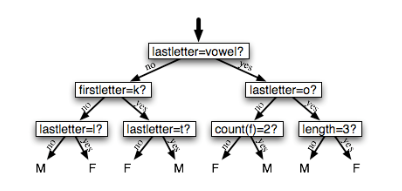
\includegraphics[width=0.5\linewidth]{images/Decisiontrees.png}
	\caption{Decision trees model to classify the gender of the names.}
	\label{fig:Decision_tree}
	\source{\url{http://www.nltk.org/book_1ed/ch06.html}}
\end{figure}

\subsection{Classification Scoring Metrics} \label{scoringmetrics} \label{metricsofclassification}

The performance of the classification model should be tested when the classification model is built. One way is to check the accuracy of the model, which is number of correct prediction out of all predictions \ref{eqn:accuracy}. 


\begin{equation}
\label{eqn:accuracy}
accuracy = \frac{correct predictions}{number of predictions}
\end{equation}

However, classification accuracy alone is usually insufficient information to check the classifier's performance if the number of input samples is not balanced. Because even if the model's accuracy is high, the prediction is biased towards the major class. 

So, several different metrics exist for evaluating the performance of a classifier. This section presents the scoring metrics used in this project.

\begin{itemize}
 \item Confusion matrix
 
 A confusion matrix is a table used to describe the prediction results of a classifier. This table can be used to describe the performance of the classifier. For instance, For a binary classifier, the table has 2 rows and 2 columns. The columns represent observed labels and the rows represent the predicted labels, shown in table \ref{tab:confusionmatrix}.
 
 \begin{itemize}
     \item True Positive($TP$) : When the prediction is positive and it’s true.
     \item False Positive($FP$) : When the prediction is positive and it’s false.
     \item False Negative($FN$) : When the prediction is negative and it’s false.
     \item True Negative($TN$) : When the prediction is negative and it’s true.
 \end{itemize}
 
\begin{table}[]
\centering
\begin{tabular}{lllll}
\cline{1-3}
\multicolumn{1}{|l|}{}   & \multicolumn{1}{l|}{Positive} & \multicolumn{1}{l|}{Negative}  &  &  \\ \cline{1-3}
\multicolumn{1}{|l|}{Positive} & \multicolumn{1}{l|}{True Positive}  & \multicolumn{1}{l|}{False Positive} &  &  \\ \cline{1-3}
\multicolumn{1}{|l|}{Negative}   & \multicolumn{1}{l|}{False Negative}  & \multicolumn{1}{l|}{True Negative}  &  &  \\ \cline{1-3}
                            &                           &                           &  & 
\end{tabular}
\caption{Confusion matrix}
\label{tab:confusionmatrix}
\end{table}
  From this table, previous known labels and predicted labels distribution can be understood, errors in prediction can be detected. In this research, confusion matrix of the both the models(migration detection and sentiment detection) is calculated to check the performance of the machine learning algorithms.
 
    \item Precision
    
    Precision is also called a positive predictive value, In binary classification, it is the number of positive prediction divided by the total number of predicted positive class values. Precision can be thought of as a measure of a classifiers exactness. It is defined in the equation \ref{eqn:Precision}. 
    
    \begin{equation}
    \label{eqn:Precision}
    Precision = \frac{TP}{TP + FP}
    \end{equation}
    
    Where $TP$ is true positive and $FP$ is a false positive.
    
    \item Recall
    
    The Recall is another performance metric in binary classification, is defined as, the number of positive predictions divided by the number of positive class values in the test data. It can be thought of as a measure of a classifiers completeness. It is shown in equation \ref{eqn:Recall} 
    
    \begin{equation}
        \label{eqn:Recall}
    Recall = \frac{TP}{TP + FN}
    \end{equation}
    
     Where $TP$ is true positive and $FN$ is a false negative.
    
    \item F1-score
   
    Which is also called as F-measure, this weights precision and recall evenly, and is given in the equation \ref{eqn:F1}.
    
        \begin{equation}
        \label{eqn:F1}
    F1 = \frac{2 * recall * precision}{precision + recall}
    \end{equation}
    In this research, the F1 score is calculated to understand the performance of the model along with its accuracy.
\end{itemize}

\subsection{Annotations}

Annotation in machine learning is the process of labeling the data, which could be in forms like images, text, audio. For example, an image can be labeled as portrait or a landscape. The computers can learn to recognize patterns and classify new data to the corresponding labels using annotated data. Annotation is usually done manually by humans, moreover, crowdsourcing can speed up the process and spread out the workload. An example of crowdsourcing is Amazon Mechanical Turk \footnote{https://www.mturk.com/}, which can be used for carrying out annotations task. This technique of using crowdsourcing to annotate emotions in the tweets was used by \cite{Mohammad:2010:EEC:1860631.1860635}. But this crowdsourcing should be compensated for their task, due to this reason in this research, I shared my dataset with my colleagues for annotation, who understood English language. The tweets were annotated by each annotator, and the mean those annotations were taken as the final label.  

\subsection{Tools}
In order to realize this research, Python programming language, and many other external tools and libraries are used. Python is an extremely powerful tool, also it is open source and flexible which adds to its popularity. It is known to have massive libraries for data manipulation and is extremely easy for all data analysts to learn and use. Some of the important libraries which are used in this research are discussed in the following section.  


\begin{itemize}
    \item NLTK \\
    NLTK(Natural Language Toolkit) is one of the most important platforms for building Python programs to work with human language data. It has comprehensive API documentation plus it provides libraries for classification, tokenization, stemming, word frequency. This library was used to generate the word cloud using the word frequency. The word cloud is an image composed of words used in a particular text, in which the size of each word indicates its frequency or importance.
    
  
    \item Scikit-learn: \\
    It  \cite{scikit-learn} is a free software machine learning library for python programming language. It is a tool for data pre-processing and data analysis, and offers many machine algorithms as well. The Scikit-learn project aims to provide state-of-the-art implementations for a wide range of machine learning methods, it has a clean API that is robust, fast, easy to use, comprehensive and well documented. The Document provides more detailed information to the experienced data analyst, while at the same time simple, key points of a topic to the beginner. Some key elements of the framework are illustrated below.
    
    \begin{itemize}
        \item Countvectorizer
        \item Feature union
        \item train test split
    \end{itemize}
    
    
 
    
    \item Pandas \\
   Pandas \cite{pythonpandas} is an open source library for the Python programming language , which provide easy-to-use data structures and data analysis tools. The data can be presented in a suitable way using its Series and DataFrame data structure.
  There are several methods in this package for convenient data filtering. Pandas have a variety of tools for seamlessly performing input and output operations. Data can be read from different formats such as CSV(comma separated values), TSV(tab separated values), MS Excel, etc.



\end{itemize}



\section{Related works in mining Twitter social media data}

This section looks at the recent development in extracting migration information from textual data, data mining on Twitter data, feature engineering in text analysis and text classification algorithms.

\subsection{Literature survey}

As a starting point, we began to examine how to detect the migration event, \cite{Goergen} paper concentrates on event detection, which is mainly focused on 3 distinct parameters
known as w3 questions, "What is really happening, Where is the incident and When did the
event happen?". The authors collect the spatial-temporal data from Twitter from two different
countries. They use Names entity recognition, Geo-coordinates to identify the location. Using these
data, authors determine the "number of possible users for a shared account by calculating the
distance and velocity between tweets belonging to single account". However, human migration is not triggered on certain incidents and we did not find the need to detect the migration event. 

Later, we started examining how to detect the Twitter user is a migrant or not. Authors from \cite{Hadgu} and  \cite{Böhm2017} presents an approach to classify the Twitter user to a particular domain, for example, Researcher or Economist. Authors of \cite{Hadgu} presents a method to classify a twitter user to a specific researcher discipline. They use a seed set from the computer science conference and crawl Twitter to collect relatively good ground truth data. This mapping is used to learn a model for classifying the Twitter user to particular desired discipline. Authors of \cite{Böhm2017}  extends this approach to classify Economist in Twitter. Their approach differs from \cite{Hadgu}, as they use the "Text" of the tweets for classification. They collect ground truth data by comparing the Twitter user account name with the economic publication database. This data is used to train a classifier model. But, In this research, It is very difficult to get the ground truth data, there is limited data where the Twitter user can be verified to figure out the Tweet is coming from a migrant or Tweet "Text" is related to migration. 
 
\cite{Hübl} paper concentrates on "Individual and aggregate trajectories that reflects the refugee migration
movements" and "identify the spatio-temporal event clusters of refugee-related tweets to
likely determine the location of refugees". The technique used by authors to collect data is, they
downloaded all the Twitter data in a specific time frame and apply filters to separate out tweets
which were of geographic interest. Authors collect both tweets which were geotagged with coordinates
and with geotagged with a place description. For the latter type, The twitter places were
are extended over continents. In addition to the above filtering method, the authors also filter tweets
of interest based on hashtag search. \cite{Hübl} work inspired me on how to collect word list for filtering
tweets related to migration. But this work was related to the refugee crisis.
 
Compare to the data collection method used by \cite{Hübl}. The authors of \cite{Cortis} use hashtag filtering
along with popular terms used in those tweets. \cite{Cortis} tries to analyze cyberbullying tweets in trending
world events. The authors choose two world events which were the cause of several cyberbullying instances.
The technique used by authors to collect and filter Twitter data is that they select two real-world
events trending hashtags along with popular cyberbullying terms. This technique inspired me to
apply this filtering logic to collect tweets regarding migration.


Regarding text classification there are two approaches, One approach is to use the labeled texts and use supervised machine learning algorithm is  trained on the labeled text data to classify the classes
of new texts. Another approach creates a sentiment lexicon and scores the text based on some function that describes how the words and phrases of the text match the lexicon, \cite{DBLP} Evaluates word list sentiment analysis for microblogging.

 \cite{Jamie} Discusses how a classifier model is trained
and evaluated by calculating precision, recall and F1 score on manually annotated and classifier
predictions.




\chapter{Approach}\label{chap:approach}
This section is a point by point depiction of the actualized framework utilized in this thesis, which is to detect the Tweets related to Human Migration  and its Sentiment. To start with, the undertaking of Mining Twitter data is defined, and next the framework is depicted in the sequential order of its working.

\section{Problem Formulation}

Predicting the topic of the Tweet is a very challenging work. People discuss or communicate all type of topics from "trending science research" to "current politics" and from "sports events" to "natural calamities" using Twitter. The topics are generic and identifying a specific topic which we need is hard to find from the tweets. The  
Principle point of this approach is a technique to identify the tweets regarding the topic ``human migration". This technique is used to  collect the tweets and build a classification model which classifies the new tweets into migration class or otherwise. And then sentiment of these tweets is detected using a sentiment detection model. The solution to the problem can be broken down into stages: Twitter data mining, feature engineering, training, and evaluation stages.


\begin{itemize}
  \item  The first stage, Data is mined from the Twitter. Data mining is a process of extracting information (with intelligent methods) from a data set and transform the information into a comprehensible structure for further use. Here, in this research, information related to human migration from Twitter dataset is extracted. However, identifying the "human migration" topic in the tweet is difficult, because ground truth value is unknown, collected tweets data cannot be mapped and searched with any population registers. The term "ground truthing" refers to the process of gathering the proper objective data for the test. So, for this reason, data are mined with respect to particular reason namely war, education or work etc. The factors which affect people for migration mentioned in the link.  \footnote{\url{http://www.bbc.co.uk/schools/gcsebitesize/geography/migration/migration_trends_rev2.shtml}  }. The four main important factors which affect human migration are:


\begin{enumerate}
    \item Economic
  \item Social
    \item Political
  \item Environmental
\end{enumerate}
Collecting an unbiased data for all the factors is very difficult. So, only political migration factor is considered in this experiment. The reason only this factor is considered because,  For instance, people can migrate for short period of time for education or work, in this scenario collecting the data from the "LinkedIn" would be more feasible as people would store and share their education and work qualification information. However, Twitter is used by many people who communicate about political issue and sufficient amount data can be collected if Twitter is used.
  
  \item In the Second stage, Meaningful features are extracted from Twitter's JSON data. There are many metadata in Tweet, such as tweet text, created date, user description and hashtags, among them text of the tweet along with the "user description" are used as a feature and additional features which are calculated using the text of the tweet like migration index, migration percentage are added to feature set. Calculation of migration index and migration percentage is mentioned in subsection below.
  
   \item The Tweets are manually annotated as migration tweets (with labels "yes" or "no"), which is used a target labels. The supervised classifier is then trained
using these feature and their corresponding labels in the training stage. Output of this model is fed to another sentiment detection model, which is trained with annotated data \cite{stanford_data}("positive" and "negative" labels) \footnote{\url{http://help.sentiment140.com/for-students/}}
  
  \item In the Fourth stage, These models are evaluated by calculating the Accuracy and the F1 score. Detailed version of evaluation is mentioned in the Evaluation section below.
\end{itemize}



\section{Method}
This section describes the method used in this research. The overview of the research is shown in the figure \ref{fig:flowchart_thesis}. The flowchart in the figure \ref{fig:flowchart_thesis} describes us that the approach is divided in to two parts. First part(left box of the figure \ref{fig:flowchart_thesis}) classifies the tweets as migration tweets. The second part(right box of the figure \ref{fig:flowchart_thesis}) is detecting the sentiment of tweets. Both the parts use the Twitter data. The output of the first model which are migration tweets are passed to second model to understand its sentiment which is shown by the arrow from left box to right box. Details of each step is mentioned in following subsections.

\begin{figure}
	\centering
	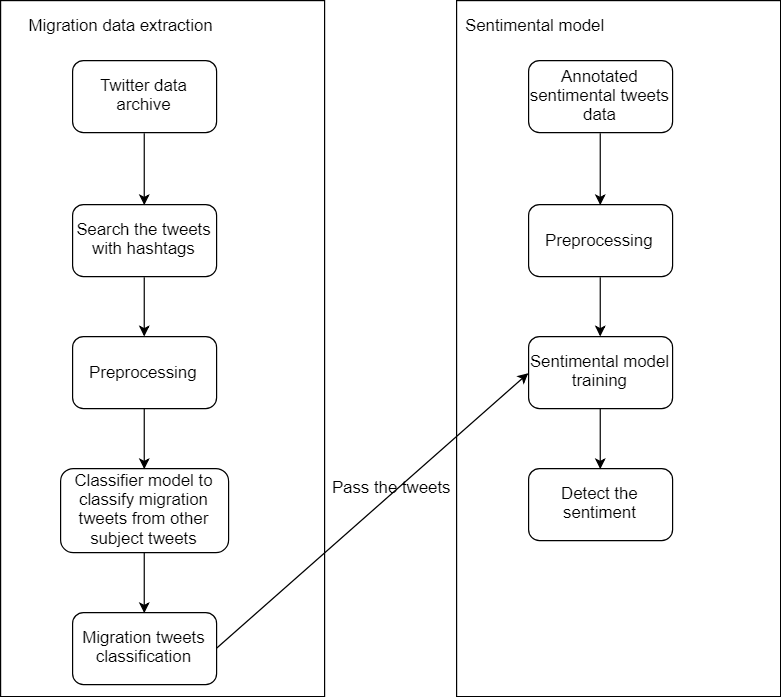
\includegraphics[width=0.75\linewidth]{images/flowchart.png}
	\caption{Flowchart of the approach}
	\label{fig:flowchart_thesis}
\end{figure}
\subsection{Data Collection}
The Twitter company offers various methods for accessing its data. They provide API's(Application Programming Interface) to access data which are of two types such as Rest API's and Streaming API's. Their applications and limitations are mentioned in section (2.1.1). The REST API offers a simple interface and is easy to use for the Twitter functionality. These API's can be used to search for already published tweets, historical tweets. Twitter's streaming API's can be used to search for the tweets which are published in current time. This API's are usually used in innovative way to collect huge number of tweet data. For instance the streaming API can be used to collect the data of any live events and this data can be used to study statistics of people attending or not attending. However, problem with these two types of API's is, it does not give full access to collect all the public tweets, they offer limitaions in accessing the data \footnote{\url{https://developer.twitter.com/en/docs/basics/rate-limiting}}. For full access of the public tweets, a commercial packages need to be purchased. The limitations and for the lack of full access of the data, helped me to decide to use the Twitter data archive which is provided in links \footnote{\url{https://archive.org/}} \footnote{\url{https://archive.org/details/twitterstream?and[]=year\%3A\%222016\%22}} \cite{Twitterarchive}. 

The archive.org is non-profit company, it is trying to build digital library of internet sites and cultural artifacts in digital form. The data from this website is free to access and is available for researchers, historians, scholars and the general public. The advantage of using data from this website is, the data can be searched and filtered according to time. for example in this research, November and December months archives from the year 2016 is considered to mine data. 

Once the data archive is chosen, next step searching for the relevant data. But, what is relevant data? for an instance, if the model built, is for ``spam email detection", it cannot be built using the data which is used for detecting ``cancellation of flights". November(2016) and the December(2016) months archives was used. This was used because the hashtags which are used were trending. Another reason why only these  two months archives used was, the same hashtags were also applied to search for tweets from other months archives, it did not result in sufficient number of tweets. Now, other questions arises is how were the hashtags chosen?. Before we choose hastags, important point to understand is why people migrate. This is discussed in chapter 3.1 in problem formulation section and only the ``Political" factors are considered in this research and in these factors, war and/or elections are the primary influences for people migrating to different countries. Based on this assumption(political factor), a significant amount of research is done studying these specific topics from news media like online news website and Twitter's trending API's and based on these studies the trending hashtags related to the topics were chosen. Hashtags chosen were ’\#refugee’, ’\#wall’, ’\#Syria’, ’\#syrianrefugee’, ’\#mexicanwall’, ’\#trumpwall’, ’\#immigrants’ and were used as the query parameter to search for tweets. 

The data in the archive is available as a JSON structure. The JSON structure of the tweet is described in section above \underline{mentioen the above section}. Archive contains all the tweets which is published in selected time. When the structure of the archive is analysed, Every line in the file was a tweet object which is in JSON format. Twitter's JSON data contains many metadata one such is `entities' metadata. This metadata contains arrays of common things in Tweets such as hashtags, user mentions, links, stock tickers (symbols), Twitter polls, and attached media. Structure of the entities metadata is shown in the figure \ref{fig:entities}. The hashtags metadata contains all the hashtags which is used in tweet's text. This structure can be used to search for the hashtags in the tweet. This idea is applied to filter tweets matching the list of hashtags which were chosen. So, a script was designed which take each line of the JSON file as the input and search the ``entity" metadata for the presence of the pre-collected hashtags list. If a match is obtained, the tweet object is stored in a csv file. One more query paramater which is used for searching filter is the language of the tweet, only ``English" language tweet were searched. This was performed by checking the ``Lang" metadata in tweet JSON obejct. The Flowchart of the tweets filter is shown in the figure \ref{fig:tweetsfilter}.


\begin{figure}
	\centering
	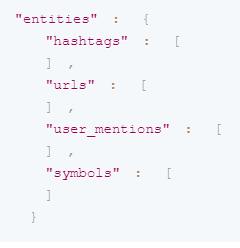
\includegraphics[width=0.5\linewidth]{images/entities.png}
	\caption{Entities metadata in tweet's JSON}
	\label{fig:entities}
\end{figure}

\begin{figure}
	\centering
	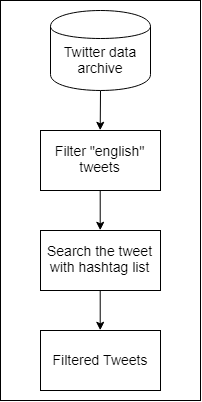
\includegraphics[width=5cm\linewidth,height=7cm]{images/filtertweets.png}
	\caption{Flowchart of the tweets filter.}
	\label{fig:tweetsfilter}
\end{figure}


\paragraph{Datasets}
The dataset has been acquired through the filtering process shown in the figure \ref{fig:tweetsfilter}. The dataset contains 1276 tweets collected using the hashtag list (’\#refugee’, ’\#wall’, ’\#Syria’, ’\#syrianrefugee’, ’\#mexicanwall’, ’\#trumpwall’, ’\#immigrants’). Hereinafter this dataset is referred to as the migration dataset. Each tweet is pre-classified manually as migration ``yes" and migration ``no" classes, in addition, the sentiment of these tweets is also annotated with ``positive" and ``negative" classes. Only two classes are selected, because binary classifier model is built using this. Text classification techniques usually have a third class ``irrelevant" or ``neutral" class. In my research, however, the third class is not considered for the reasons, number of tweets in the data set is smaller and if the third classes is chosen some data is lost. Moreove, while annotating if the tweets belong to the ``irrelevant" or ``neutral" class, they are classified to ``negative" class. The classes of the tweets in this dataset are annotated by my colleagues who understand and speaks english fluently. The dataset was shared with five of my colleagues and the average of the annotation was the considered as the final class. The distribution of the two classes `yes' and `no' classes is show in the figure \ref{tab:DistMigrationClass}. The distribution of the two classes `positive' and `negative' classes is show in the figure \ref{tab:Distribution of sentiment class}.



\begin{table}[]
\centering
\begin{tabular}{lllll}
\cline{1-2}
\multicolumn{1}{|l|}{Classes}   & \multicolumn{1}{l|}{number of tweets} &  &  &  \\ \cline{1-2}
\multicolumn{1}{|l|}{``yes"} & \multicolumn{1}{l|}{449}  &  &  &  \\ \cline{1-2}
\multicolumn{1}{|l|}{``no"}   & \multicolumn{1}{l|}{826}  &  &  &  \\ \cline{1-2}
                            &                           &  &  & 

\end{tabular}
\caption{Distribution of migration class}
\label{tab:DistMigrationClass}
\end{table}

\begin{table}[]
\centering
\begin{tabular}{lllll}
\cline{1-2}
\multicolumn{1}{|l|}{Classes}   & \multicolumn{1}{l|}{number of tweets} &  &  &  \\ \cline{1-2}
\multicolumn{1}{|l|}{``positive"} & \multicolumn{1}{l|}{565}  &  &  &  \\ \cline{1-2}
\multicolumn{1}{|l|}{``negative"}   & \multicolumn{1}{l|}{710}  &  &  &  \\ \cline{1-2}
                            &                           &  &  & 
\label{tab:Distribution of sentiment class}
\end{tabular}
\caption{Distribution of sentiment class}
\label{tab:DistsentimentClass}
\end{table}

Beside the migration dataset, two additinal dataset is collected. First, for sentiment detection model and second, for evaluation of the classification model for migration. For the Sentiment detection model, annotated sentiment data from \cite{stanford_data} is used. This dataset contains 1.6 million tweets, of which it contains  800000 tweets of each class. This data is cleaned and sentiment classification model is built. Another dataset is collected is from \cite{CanadianmMigrationDataset}. This is a dataset for Canadian migration collected on Twitter. This dataset contains 800 tweets which are classified into migration tweets, for which additional 800 random tweets are added to balance the data set. The 800 additional tweets are classified as non-migration tweets. For this dataset, the migration dataset is added and the accuracy of the model built with combined dataset is compared with the accuracy of the model built with migration dataset. 



\subsection{Pre-processing}
The overall system output standards depend on the quality of the input data. The additional information provided by Twitter data(example: user mentions, url's) does not provide many useful properties. Hence to enhance the quality  of the input information a pre-preparing stage is required. The pre-processing step applies to all three collected data sets. Since the data sets only contain Twitter data, the preprocessing step is common for all data sets. Pre-processing process involves many steps: language check, removal of duplicate , merging tweet message and user description, message cleaning which is show in the figure \ref{fig:preprocessing}. 

The tweets in the dataset are present in JSON format, so each line of the file is a JSON object. The preprocessing script reads the file line by line, parses each line into JSON object and acts as follows.

\subsubsection{Language check}
Since Twitter is used worldwide, the messages are generally available in almost any language. Text analysis and classification makes use of linguistic content and language therefore language plays a key role. The Language importance in any text classification is discussed in the section \ref{chap:background}. In this research, I restrict my scope to tweets in English only. Non-English tweet messages are therefore discarded before any experimental steps performed on the dataset. 
Language detection is one of the interesting and challenging field in Natural language processing(NLP). Researches use translators to convert the message to a single language for text analysis, usually to English.
\begin{figure}
	\centering
	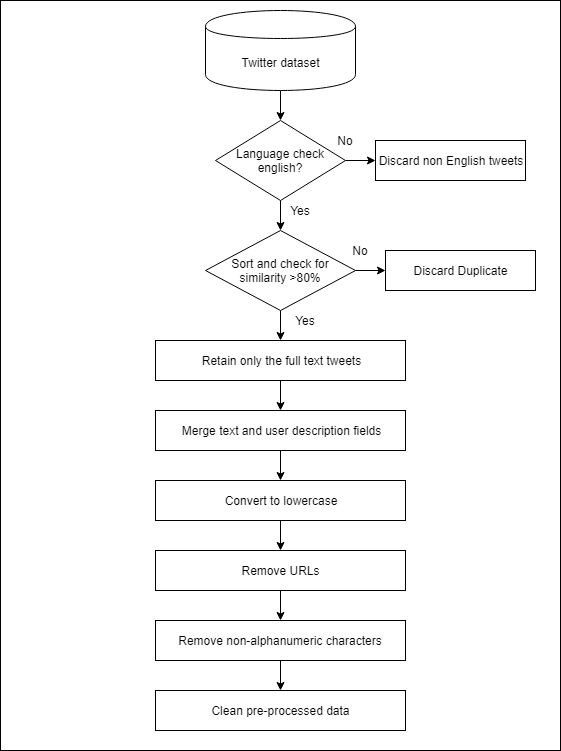
\includegraphics[width=10cm\linewidth,height=13cm]{thesis_template/images/preprocessing.png}
	\caption{Pre-processing steps}
	\label{fig:preprocessing}
\end{figure}
However, to implement language check and to filter only English language tweet messages. I take advantage of the Twitter data structure. Twitter stores each message as a JSON object and it contains ``Lang" metadata which  informs that, to which language the message belongs to. A script is implemented to check this, before the tweets are passed on to the next pre-processing stage. This script checks the ``Lang" metadata for the keyword ``en" which signifies the language is English and discards other keywords(Example, ``es" for Spanish , ``jp" for Japanese). By the end of this script only English tweets are collected passed on to duplicate message checking step.  

\subsubsection{Removal of duplicate messages}
After the Language filter, next step which is used in research is duplicate check of the tweet messages. There is a lot of research on the use of duplicates in the data set in the field of data science. There is no hard rule to remove the duplicates in the dataset. Sometimes the machine learning model improves the accuracy, and at times  the model is over-fitted. Since, word frequency is used in this research, allowing the duplicate message simply increases the word count and the classifier model
achieves a very low training error by learning to be very good at same data that repeats a lot in the training set.

Another important reason why duplicates need to be removed especially in this research is, the Twitter's functionality of ``re-tweeting". A retweet is just a repost of the tweet of another Twitter user on your own profile. Like hashtags, retweets are a community - driven phenomenon on Twitter that helps to improve the service and make it easier for people to talk. So after searching the tweets with hashtags and filtering only english tweet, duplicate messages tweet is implemented.

This duplicate checker is implemented using a simple idea to sort the text of tweets first and to compare two consecutive texts for similarity. The two consecutive texts shall only be considered similar if they are 80\% similar. If the two tweets are similar only tweet is saved and other tweet is discarded. Flowchart of the process in shown in the figure \ref{fig:duplicatechk}. Sorting and similarity check is implemented using the `pandas' python library\footnote{\url{https://pandas.pydata.org/pandas-docs/version/0.17.0/generated/pandas.DataFrame.sort_values.html}} and `difflib' python library \footnote{\url{https://docs.python.org/2/library/difflib.html}}.

\begin{figure}
	\centering
	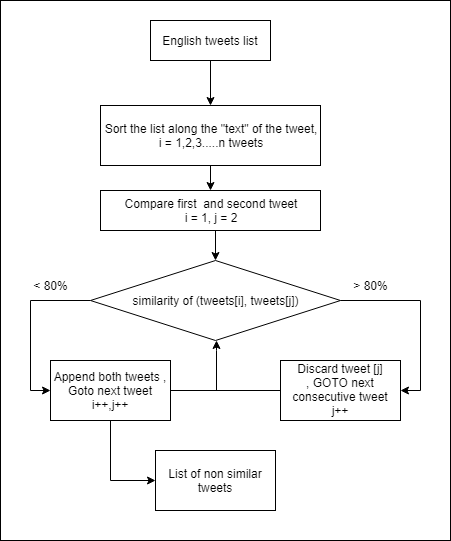
\includegraphics[width=10cm\linewidth,height=10cm]{thesis_template/images/duplicatecheck.png}
	\caption{Removal of duplicate messages}
	\label{fig:duplicatechk}
\end{figure}

\subsubsection{Merge text and Description fields}

One element which made Twitter popular social media network is that it limits your posts to 140 characters(recently characters length is increased to 280). However, this could be disadvantageous for data scientists who try to extract information from the tweet message. Since only 140 characters and people try to shorten the message using acronyms and a lot of unwanted information is also present in a tweet which includes url and users mention. This research therefore combines the text of the tweet message with a user description, which increases the number of characters. User description is another metadata which is present in Twitter JSON structure. In addition, I could just get some more information about user migration by including his/her description. This implement is a simple task, a script just checks whether the user description field has a value if present it is merged with the message.

\subsubsection{Message cleaning}
In this step, the text in the tweet message is cleaned. The message of the Tweet contains only 140 characters, To this user description is added. But, as mentioned before, This limited size constraints make people to shorten the message using acronyms and wrong spelling. 
In order to create a purer data set for the classifier training, message cleaning techniques are used. First, all the characters are converted to lowercase. Once it is normalized into single basic structure, several techniques are applied such as remove URL's, remove non-alphanumeric characters. This is implemented using the regular expression, which is a efficient string replacement algorithm. Another actions was performed was removal of the stop words. Stop words are the commonly occuring words(such as "a", "the", "is", "in") because it just adds the number of words and provide less information. also takes processing time. This was done using the NLTK library which is available in python language, it has the stopwords list of for 16 different languages. 
\subsubsection{Manual Annotations}
The Data-sets collected are shared with three of my colleagues to annotate. Each annotator annotates the tweet with 2 labels. One as migration "yes" or "no" and second for the sentiment of the tweets "pos" or "neg". I take a mean of those annotations and assign the labels for each collected tweet.

\subsection{Feature engineering} \label{featureengineering}


 
Before classifying tweets using the machine learning approach, features must be extracted after the pre-processing step. Without the right set of features, even the powerful machine learning algorithm results badly. This was understood from the literature survey. As mentioned in problem formulation section, I am building two separate models, and both the models follow same feature extraction methods, but for the migration tweets classifier model has two additional features.

In my research, I have created a heterogeneous feature set. Heterogeneous feature set advantages are discussed in \ref{chap:background}. Feature set contains, features extracted from the text using count vector technique, and additional two feature are added to this feature, that is ``Migration index" and ``Migration percentage".   

I decided to create a feature vector using count vectorizer. This technique is simple to implement and decision to use this was based on the performance. The count vector is implemented using the "CountVectorizer" library from scikit learn \cite{scikit-learn}. The CountVectorizer library offers a simple way to tokenize a collection of text documents and build a vocabulary of known words, but also to encode new documents using that vocabulary. This library takes text document as input and to learn about the document a fit function is executed. Then an encoded vector with an entire vocabulary length and an integer count for the number of times each word appeared in the document is returned. The returned vector is a sparse as it contains many zeroes. This sparse matrix is handled using sparse library from scipy.org.

Migration index" is computed based on the Dictionary. This dictionary is a list of words which are related to migration along with corresponding weights which are manually assigned based on the severity level which is 1 to 5, 1 being negligible and 5 being extremely related to migration. This severity is calculated based on the word frequency. A word-cloud is generated with the collected tweets "text" and the severity number is assigned to the words based on the most frequently occurring word.
 I check all the tweets for the presence of words from this dictionary if present it gets the corresponding weights of all those words and mean is calculated for those weights. This mean value is "Migration index". 
 


Presence of Migration term in tweet message alone cannot necessarily mean the text is related
to Human migration. The text/tweet can be considered more related to migration if the migration word is directed at a particular individual, a group of
people, race, country, religion etc. For this reason, I also created a list of pronouns and collective nouns, with this ”Migration percentage” is calculated based on the presence of Migration word along with pronouns or collective nouns.




Finally, the Count vector feature, migration index, migration percentage are combined and used a feature set, which is shown in the fig \ref{fig:featureeng}. This set and its corresponding classes are split in test and training set, and used as a input to supervised machine learning algorithm, which is discussed in the next section.

\begin{figure}
	\centering
	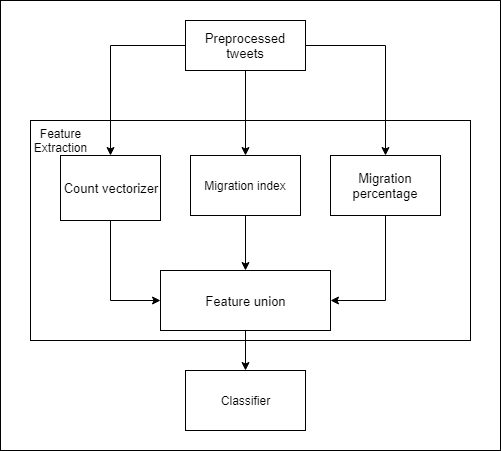
\includegraphics[width=10cm\linewidth,height=10cm]{thesis_template/images/featureengineering.png}
	\caption{Migration model feature engineering}
	\label{fig:featureeng}
\end{figure}
    

Location is obtained using the "Geopy" python library. The user location is passed to "Geopy" library to get latitude and longitude. 



\subsection{Dataset split}
Before we can train any model, we think about how to split the data first. There are two types of splitting the data such as:
\begin{enumerate}
    \item Test/Train sets
  \item Test/Train/Dev sets
\end{enumerate}
The definitions of the three terms are as following:
\begin{itemize}
     \item Train set: Sample of data used of learning.
 
    \item Test set: Sample of data used for calculating the accuracy of model.
      \item Dev set: Sample of data which is used for unbiased evaluation of the model performance.
\end{itemize}

From now on I will be discussing about the two models, firstly migration detection and second, sentiment detection. For the migration detection model, I decided to divide the data set in test and train sets for the migration detection model, Because there were fewer tweets. It was split as 75\% train and 25\%test sets. The data is divided into test, train and dev sets for the sentiment detection model, because more tweets are available and this was split as 98\% train set, 1\%test set, and 1\% dev set.
Distribution of the Tweets after the train/test split for migration dataset is shown in the table \ref{tab:Distmigrationdataset}. Distribution of the Tweets after the train/test/dev split for sentiment dataset is shown in the table \ref{tab:Distsentimentdatset}. This split was implemented using the ``modelselection" library from the scikit learn \cite{scikit-learn}.


\begin{table}[]
\centering
\begin{tabular}{lllll}
\cline{1-2}
\multicolumn{1}{|l|}{Sets}   & \multicolumn{1}{l|}{number of tweets} &  &  &  \\ \cline{1-2}
\multicolumn{1}{|l|}{Train} & \multicolumn{1}{l|}{956}  &  &  &  \\ \cline{1-2}
\multicolumn{1}{|l|}{Test} & \multicolumn{1}{l|}{319}  &  &  &  \\ \cline{1-2}
\multicolumn{1}{|l|}{Total}   & \multicolumn{1}{l|}{1275}  &  &  &  \\ \cline{1-2}
                            &                           &  &  & 
\label{tab:Distribution of sentiment class}
\end{tabular}
\caption{Distribution of train/test split for migration dataset}
\label{tab:Distmigrationdataset}
\end{table}

\begin{table}[]
\centering
\begin{tabular}{lllll}
\cline{1-2}
\multicolumn{1}{|l|}{Sets}   & \multicolumn{1}{l|}{number of tweets} &  &  &  \\ \cline{1-2}
\multicolumn{1}{|l|}{Train} & \multicolumn{1}{l|}{1568000}  &  &  &  \\ \cline{1-2}
\multicolumn{1}{|l|}{Dev} & \multicolumn{1}{l|}{16000 }  &  &  &  \\ \cline{1-2}
\multicolumn{1}{|l|}{Test} & \multicolumn{1}{l|}{16000 }  &  &  &  \\ \cline{1-2}
\multicolumn{1}{|l|}{Total}   & \multicolumn{1}{l|}{1600000}  &  &  &  \\ \cline{1-2}
                            &                           &  &  & 
\label{tab:Distribution of sentiment class}
\end{tabular}
\caption{Distribution of train/dev/test split for migration dataset}
\label{tab:Distsentimentdatset}
\end{table}


\subsection{Classification}
As mentioned above, this project incorporates two classifier models. One, migration detection classifier, another model for sentiment detection. The tweets classified as migration tweets are transferred to the second model in order to detect their sentiment. The feature extraction method is slightly different for both models. For the migration model, the feature set contains a tweet message count vector, migration index, and migration percentage. However, the sentiment detection model contains only the tweet message count vector as a feature set. So, these feature set are passed as the input to the classifier. To classify tweets, there are many algorithms. However, I have compared the accuracy of three classifier algorithms, such as naive Bayes, logistic regression and decision trees. The classifier learns a pattern based on the inputs and classifies new samples into specific classes.



\subsection{Evaluation}

Two types evaluation is conducted in this research,
\begin{enumerate}
    \item To evaluate the migration detection model. This is conducted by 2 methods:
    \begin{itemize}
        \item First method : 
        Evaluate the classifier model by splitting the data with
        test and train data set, as the ground truth is manually annotated. And then calculating the F1 score on the "Test data set".
        \item Second method :
        \begin{itemize}
            \item With Canadian migration data [2], which is a migration-related dataset where each tweet in the dataset belongs to migration (label "yes"). A subset (1000 tweets) will be taken at first, along
            with 1000 tweets which belong to general categories where these tweets are manually picked which are not related to migration (label "no"). 
            \item With these 2000 general and Canadian tweets, Another set of tweets which are collected from the hashtags from the data- collection step are combined together totaling to 3000 tweets.
            \item A binary classifier will be trained from the above tweets, and the accuracy of this model and the model which is built only from the prepossessing step is compared. To check whether the model with manually collected and annotated tweets perform better or the model with other migration data classifier.
        \end{itemize}
        
    \end{itemize}


    \item Evaluating the Sentiment analysis is performed with the "test data set",
by calculating the F1 score, Accuracy.
\end{enumerate}
\include{chapters/method}
\chapter{Experiment}\label{chap:experiment}

Three sets of experiments have been conducted. A migration tweet detection was executed at the beginning of the project, exploring the performance of the three classifier. A sentiment detection model is built using annotated data, performance metric are computed. Tweets which are classified as migration tweets are passed to sentiment detection model to detect its sentiment.

\section{Migration detection model}
This section describes the steps which were conducted while building migration detection model.
\subsection{Data-set collection}

For the migration detection model, twitter archives \footnote{\url{https://archive.org/}} was considered to collect the data.
The data-set was collected by filtering out, using following hash-tags
\#refugee, \#wall, \#Syria, \#syrianrefugee,
\#mexicanwall, \#trumpwall, \#immigrants. A total of 1275 tweets were collected from data archive(100GB). The year 2016 was chosen because the hash tags used to search tweets were trending during that period. The tweets filtered are stored in JSON format.



\subsection{Prepossessing} \label{sssec:preprocessing}

Data prepossessing is fundamental step to all data science and
Natural Language Processing Tasks. The prepossessing steps in
our project is common to both migration detection and sentiment detection models the models. After retrieving the JSON, the prepossessing script performs the following steps:
\begin{enumerate}
    \item Take only lines with "English" language Tweets.
    \item Sort the tweets, Check similarity between consecutive tweets , if similarity is greater than 80\%, remove the duplicate tweets.
    \item Search for the full\_text of the tweet (In cases of re-tweets or too big tweets, additional attributes are added to the tweet.
    \item Deleting all non-alphanumeric characters.
\end{enumerate}
The scripts are mainly implemented using the regular expression. The prepossessed tweets are manual annotated with label ``yes" and ``no". After this step the data is clean and is passed to feature engineering step. Distribution of obtained tweets are show in the figure \ref{fig:graphDistmigration}.

\begin{figure}
	\centering
	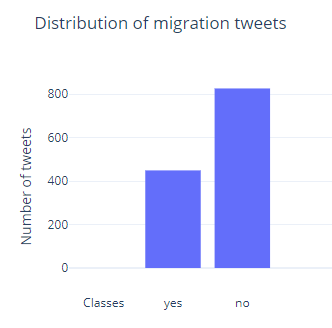
\includegraphics[width=10cm\linewidth,height=10cm]{thesis_template/images/distofmigration_tweetsundefined.png}
	\caption{Distribution of the migration tweets}
	\label{fig:graphDistmigration}
\end{figure}


\subsection{Feature engineering }
Feature Engineering starts from an initial set of measured data and
build derived values (features) which is intended to be informative. In this project, Count vectorizer is used to extract feature from the text of the tweet. Along with that Migration index(MI) and migration percentage(MP) is calculated, section \ref{featureengineering} discusses the process of computing MI and MP. Count vector is a sparse matrix, this feature is combined with MP and MI feature using feature union technique, section \ref{backgroundworkFeatureEngi} discusses the technique of feature union.  

\subsection{Classification and Metrics}
The classifier is treated as a binary classifier, with the labels ``yes" and ``no". The label ``yes" represents the tweets is a migration tweet and the label ``no" represnts the tweets is not related to migration. For classification results in any classification analysis, accuracy, precision, recall and F1 are computed. Since the F1 score is a harmonic means of precision and recall, it is sometimes enough to report this metric. In our experiments, we follow this convention and report all the above measurements and a macro- averaged F1 score.

Three classifier are used in this project, naive Bayes, Logistic regression, decision trees. Performance metric of all the three classifier is given in table \ref{tab:Migration_metric}


\begin{table}[]
\centering
\begin{tabular}{lllll}
\hline
\textbf{Classifier} & \textbf{Accuracy} & \textbf{Precision} & \textbf{Recall} & \textbf{F1-score} \\ \hline
Logistic regression & 0.937             & 0.956              & 0.844           & 0.896             \\ \hline
Naive Bayes         & 0.821             & 0.709              & 0.757           & 0.732             \\ \hline
Decision Trees     & 0.943             & 0.938              & 0.883           & 0.909             \\ \hline
\end{tabular}
\caption{Performance metric of all the classifier - Migration model}
\label{tab:Migration_metric}
\end{table}

\subsubsection{Naive Bayes}
The performance score and confusion matrix of migration detection from the naive Bayes model is show in the table \ref{tab:confusionmatrix_migrationtweets} and \ref{tab:performancemetricofmigration}

\begin{table}[]
\centering
\begin{tabular}{lllll}
\cline{1-3}
\multicolumn{1}{|l|}{}   & \multicolumn{1}{l|}{predicted\_YES} & \multicolumn{1}{l|}{predicted\_NO}  &  &  \\ \cline{1-3}
\multicolumn{1}{|l|}{YES} & \multicolumn{1}{l|}{78}  & \multicolumn{1}{l|}{25} &  &  \\ \cline{1-3}
\multicolumn{1}{|l|}{NO}   & \multicolumn{1}{l|}{32}  & \multicolumn{1}{l|}{184}  &  &  \\ \cline{1-3}
                            &                           &                           &  & 
\end{tabular}
\caption{Naive Bayes: Confusion matrix for migration model}
\label{tab:confusionmatrix_migrationtweets}
\end{table}





\subsubsection{Logistic regression}
The performance score and confusion matrix of migration detection model using the logistic regression algorithm is show in the table \ref{tab:confusionmatrix_migrationtweets} and \ref{tab:performancemetricofmigration}

\begin{table}[]
\centering
\begin{tabular}{lllll}
\cline{1-3}
\multicolumn{1}{|l|}{}   & \multicolumn{1}{l|}{predicted\_YES} & \multicolumn{1}{l|}{predicted\_NO}  &  &  \\ \cline{1-3}
\multicolumn{1}{|l|}{YES} & \multicolumn{1}{l|}{87}  & \multicolumn{1}{l|}{16} &  &  \\ \cline{1-3}
\multicolumn{1}{|l|}{NO}   & \multicolumn{1}{l|}{4}  & \multicolumn{1}{l|}{212}  &  &  \\ \cline{1-3}
                            &                           &                           &  & 
\end{tabular}
\caption{Logistic regression: Confusion matrix for migration model}
\label{tab:confusionmatrix_migrationtweets}
\end{table}





\subsubsection{Decision trees}
The performance score and confusion matrix of the migration detection model using decision trees algorithm can be found in the table.
 \ref{tab:confusionmatrix_migrationtweets} and \ref{tab:performancemetricofmigration}

\begin{table}[]
\centering
\begin{tabular}{lllll}
\cline{1-3}
\multicolumn{1}{|l|}{}   & \multicolumn{1}{l|}{predicted\_YES} & \multicolumn{1}{l|}{predicted\_NO}  &  &  \\ \cline{1-3}
\multicolumn{1}{|l|}{YES} & \multicolumn{1}{l|}{87}  & \multicolumn{1}{l|}{16} &  &  \\ \cline{1-3}
\multicolumn{1}{|l|}{NO}   & \multicolumn{1}{l|}{4}  & \multicolumn{1}{l|}{212}  &  &  \\ \cline{1-3}
                            &                           &                           &  & 
\end{tabular}
\caption{Decision trees: Confusion matrix for migration model}
\label{tab:confusionmatrix_migrationtweets}
\end{table}






\section{Sentiment detection model}
\subsection{Data-set collection}
For the sentiment detection model, Annotated data-set from the Stanford Twitter Corpus \footnote{\url{http://help.sentiment140.com/for-students/}} was used. Distribution of the tweets is shown in the figure \ref{fig:graphDistsentiment}

\subsection{Prepossessing}
Prepossessing steps are same as mentioned in section 

fig \ref{fig:graphDistsentiment}
\begin{figure}
	\centering
	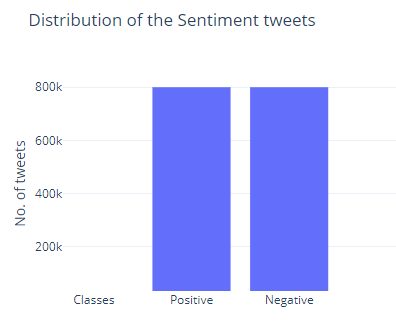
\includegraphics[width=12cm\linewidth,height=10cm]{thesis_template/images/distofsentiment_tweetsundefined.png}
	\caption{Distribution of the sentiment tweets}
	\label{fig:graphDistsentiment}
\end{figure}


\subsection{Feature engineering }
\subsection{Classification and Metrics}

\subsubsection{Logistic regression}

\begin{table}[]
\centering
\begin{tabular}{lllll}
\cline{1-3}
\multicolumn{1}{|l|}{}   & \multicolumn{1}{l|}{predicted\_YES} & \multicolumn{1}{l|}{predicted\_NO}  &  &  \\ \cline{1-3}
\multicolumn{1}{|l|}{YES} & \multicolumn{1}{l|}{6624}  & \multicolumn{1}{l|}{1294} &  &  \\ \cline{1-3}
\multicolumn{1}{|l|}{NO}   & \multicolumn{1}{l|}{1443}  & \multicolumn{1}{l|}{6599}  &  &  \\ \cline{1-3}
                            &                           &                           &  & 
\end{tabular}
\caption{Logistic regression: Confusion matrix for sentiment model}
\label{tab:confusionmatrix_migrationtweets}
\end{table}



\subsubsection{Naive Bayes}



\begin{table}[]
\centering
\begin{tabular}{lllll}
\cline{1-3}
\multicolumn{1}{|l|}{}   & \multicolumn{1}{l|}{predicted\_YES} & \multicolumn{1}{l|}{predicted\_NO}  &  &  \\ \cline{1-3}
\multicolumn{1}{|l|}{YES} & \multicolumn{1}{l|}{78}  & \multicolumn{1}{l|}{25} &  &  \\ \cline{1-3}
\multicolumn{1}{|l|}{NO}   & \multicolumn{1}{l|}{32}  & \multicolumn{1}{l|}{184}  &  &  \\ \cline{1-3}
                            &                           &                           &  & 
\end{tabular}
\caption{Naive Bayes: Confusion matrix for sentiment model}
\label{tab:confusionmatrix_migrationtweets}
\end{table}



\subsubsection{Decision trees}



\begin{table}[]
\centering
\begin{tabular}{lllll}
\cline{1-3}
\multicolumn{1}{|l|}{}   & \multicolumn{1}{l|}{predicted\_YES} & \multicolumn{1}{l|}{predicted\_NO}  &  &  \\ \cline{1-3}
\multicolumn{1}{|l|}{YES} & \multicolumn{1}{l|}{78}  & \multicolumn{1}{l|}{25} &  &  \\ \cline{1-3}
\multicolumn{1}{|l|}{NO}   & \multicolumn{1}{l|}{32}  & \multicolumn{1}{l|}{184}  &  &  \\ \cline{1-3}
                            &                           &                           &  & 
\end{tabular}
\caption{Decision trees: Confusion matrix for sentiment model}
\label{tab:confusionmatrix_migrationtweets}
\end{table}






\section{Sentiment analysis of migration classified tweets}

Tweets classified as migration tweets from the migration detection model are passed to the sentiment detection model. The migration tweets are also annotated with their respective sentiment labels in tweet annotation step. This step to annotate the sentiment of migration tweets is considered as the ground truth, and the performance of the sentiment detection model which is built using logistic regression algorithm is calculated using the ground truth and the predicted value. 
The number of tweets which are classified as the migration tweets is 449 tweets, and the distribution of the annotated sentiment labels is shown in the figure \ref{fig:sent_migration_distribution}. The performance metric of detecting the sentiment of these tweets are shown in table \ref{tab:sentiment_of_Migration_metric}

 

\begin{figure}
	\centering
	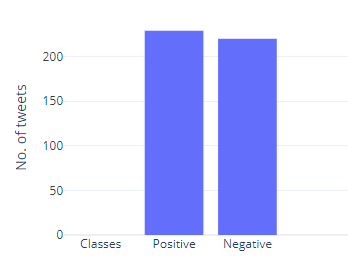
\includegraphics[width=12cm\linewidth,height=10cm]{thesis_template/images/sentiment_of_migration_tweets.png}
	\caption{ The distribution of "sentiment labels" for the classified migration tweets.}
	\label{fig:sent_migration_distribution}
\end{figure}

\begin{table}[]
\centering
\begin{tabular}{lllll}
\hline
\textbf{Classifier} & \textbf{Accuracy} & \textbf{Precision} & \textbf{Recall} & \textbf{F1-score} \\ \hline
Logistic regression & 57.02             & 0.58              & 0.57          & 0.55              \\ \hline

\end{tabular}
\caption{Performance metric of detecting the sentiment of migration tweets}
\label{tab:sentiment_of_Migration_metric}
\end{table}
\chapter{Evaluation}\label{chap:evaluation}
Once the problem is set and the data is prepared,  machine learning model is applied to solve the problem. But, The model built to solve the problem might not be good, lot of time is spend on choosing, running and tuning algorithms. One way to test the machine learning model is to, define the test harness on which the model performance can be computed. Another method is, compare the the model by adding more input samples. 

In this research, two models are built, one for the detection of migration and one for the detection of sentiment. Evaluation of sentiment detection model is discussed in Section \ref{snetimentdetectionmodel}. The migration detection model's performance metrics is discussed in the Section \ref{migration_detection_experiment}. In addition to these evaluation metrics, the migration model is evaluated by adding more samples that are not considered from the data collection step but from the other external source. Hereinafter, the new samples is called as canadian migration dataset. The technique is discussed in the section \ref{eval}. combined data is preprocessd with same series of step which was discused in Section \ref{preprocessing} . The model is built using this data with three classifier algorithm. 

The distribution of tweets after combining migration dataset and canadian migration dataset is shown in the graph \ref{fig:combined}. The confusion matrix of all the three classifier is given the table [\ref{tab:confusionmatrix_migrationtweets_com_LR},\ref{tab:confusionmatrix_migrationtweets_com_NB},\ref{tab:confusionmatrix_migrationtweets_com_DT}] and the performance metric is given the table \ref{tab:sentiment_metric_com}.

Comparing the two metric table  \ref{tab:sentiment_metric_com} and \ref{tab:Migration_metric}


\begin{figure}
	\centering
	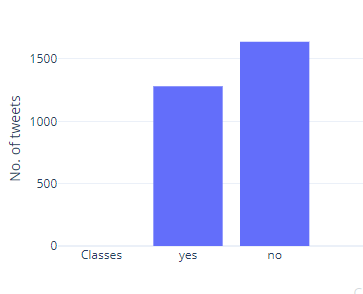
\includegraphics[width=10cm\linewidth,height=10cm]{thesis_template/images/combined.png}
	\caption{Distribution of the combined tweets}
	\label{fig:combined}
\end{figure}




\begin{table}[]
\centering
\begin{tabular}{lllll}
\cline{1-3}
\multicolumn{1}{|l|}{}   & \multicolumn{1}{l|}{predicted\_YES} & \multicolumn{1}{l|}{predicted\_NO}  &  &  \\ \cline{1-3}
\multicolumn{1}{|l|}{YES} & \multicolumn{1}{l|}{158}  & \multicolumn{1}{l|}{81} &  &  \\ \cline{1-3}
\multicolumn{1}{|l|}{NO}   & \multicolumn{1}{l|}{52}  & \multicolumn{1}{l|}{234}  &  &  \\ \cline{1-3}
                            &                           &                           &  & 
\end{tabular}
\caption{Logistic regression:Confusion matrix for migration model on combined dataset}
\label{tab:confusionmatrix_migrationtweets_com_LR}
\end{table}

\begin{table}[]
\centering
\begin{tabular}{lllll}
\cline{1-3}
\multicolumn{1}{|l|}{}   & \multicolumn{1}{l|}{predicted\_YES} & \multicolumn{1}{l|}{predicted\_NO}  &  &  \\ \cline{1-3}
\multicolumn{1}{|l|}{YES} & \multicolumn{1}{l|}{166}  & \multicolumn{1}{l|}{73} &  &  \\ \cline{1-3}
\multicolumn{1}{|l|}{NO}   & \multicolumn{1}{l|}{100}  & \multicolumn{1}{l|}{186}  &  &  \\ \cline{1-3}
                            &                           &                           &  & 
\end{tabular}
\caption{Niave Bayes: Confusion matrix for migration model on combined dataset}
\label{tab:confusionmatrix_migrationtweets_com_NB}
\end{table}


\begin{table}[]
\centering
\begin{tabular}{lllll}
\cline{1-3}
\multicolumn{1}{|l|}{}   & \multicolumn{1}{l|}{predicted\_YES} & \multicolumn{1}{l|}{predicted\_NO}  &  &  \\ \cline{1-3}
\multicolumn{1}{|l|}{YES} & \multicolumn{1}{l|}{170}  & \multicolumn{1}{l|}{69} &  &  \\ \cline{1-3}
\multicolumn{1}{|l|}{NO}   & \multicolumn{1}{l|}{70}  & \multicolumn{1}{l|}{216}  &  &  \\ \cline{1-3}
                            &                           &                           &  & 
\end{tabular}
\caption{Decision trees: Confusion matrix for migration model on combined dataset}
\label{tab:confusionmatrix_migrationtweets_com_DT}
\end{table}

\begin{table}[]
\centering
\begin{tabular}{lllll}
\hline
\textbf{Classifier} & \textbf{Accuracy} & \textbf{Precision} & \textbf{Recall} & \textbf{F1-score} \\ \hline
Logistic regression & 0.746           & 0.752              & 0.661           & 0.703            \\ \hline
Naive Bayes         & 0.670             & 0.624              & 0.694           & 0.657             \\ \hline
Decision Trees     & 0.735             & 0.708              & 0.711           & 0.709             \\ \hline
\end{tabular}
\caption{Performance metric of all the classifier - Migration model on combined dataset}
\label{tab:sentiment_metric_com}
\end{table}





% -- Appendix (optional)
\begin{appendices}
    % !TeX spellcheck = en_US
% !TeX encoding = UTF-8

\end{appendices}
\newpage


%%%%%%%%%%%%%%%%%%%%%%%%%%%%%%%%%%%%%%%%%%%%%%%%%%%%%%%%%%%%%%%%%%%%%%%%%%%%%%%%%%%%%%%%%
\backmatter

% -- Bibliography
\printbibliography

% -- Eidesstattliche Erklärung (= Affadavit)
% !TeX spellcheck = de_DE
% !TeX encoding = UTF-8

\chapter{Eidesstattliche Erkl\"arung}

	Hiermit versichere ich, dass ich diese \thesisType{} selbstst\"andig und ohne Benutzung anderer als der angegebenen Quellen und Hilfsmittel angefertigt habe und alle Ausf\"uhrungen, die w\"ortlich oder sinngem\"a\ss{} übernommen wurden, als solche gekennzeichnet sind, sowie, dass ich die \thesisType ~in gleicher oder \"ahnlicher Form noch keiner anderen Pr\"ufungsbeh\"orde vorgelegt habe.

	\vspace{3cm}

	Passau, \thedate

	\vspace{2cm}

	\parbox{8cm}{
		\hrule \strut \theauthor
	}




\end{document}